%- - - - - - - - - - - - - - - - - - - - - - - - - - - - - - - - - 
\label{sec:online}

\subsection{Data acquisition}
%\textbf{\emph{Jan B.}}

We envision a DAQ system following a streaming readout paradigm. In the following, we will describe the individual components as well as the overall data flow and bandwidth model. An overview of the system is shown in Figure \ref{fig:data_acquisition_diagram}.


\begin{figure}[hbt!]
 \begin{center}
  % \raisebox{0.5mm}{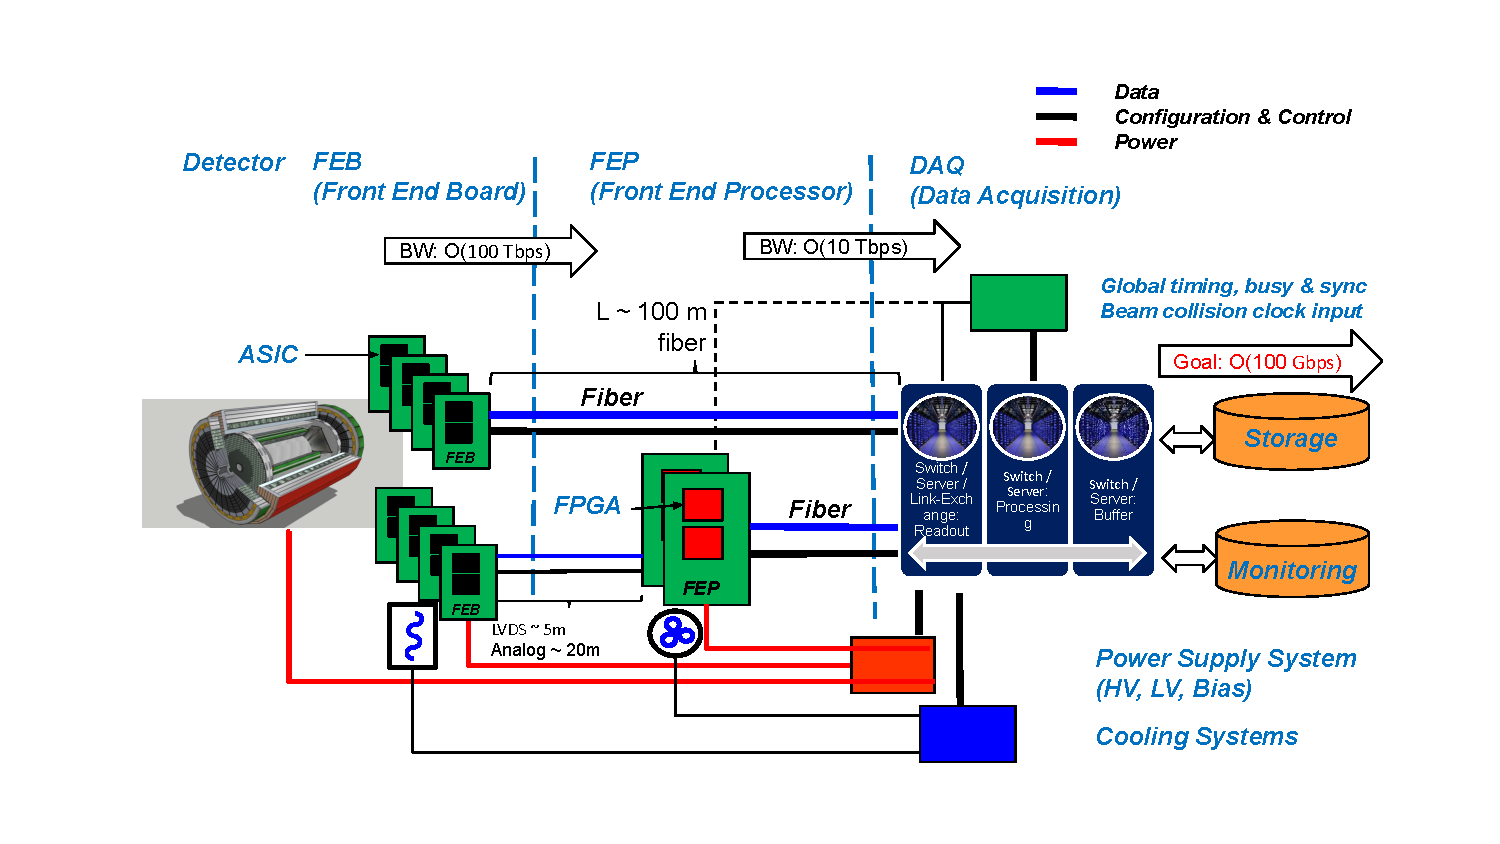
\includegraphics[trim=50 30 50 30, clip, width=0.99\linewidth]{figs/figure_data_acquisition_diagram.pdf}}
  \usetikzlibrary{arrows,chains,shapes,matrix,scopes,positioning,fadings,backgrounds,fit,mindmap,trees,decorations.markings,decorations.pathreplacing,calc}
\usetikzlibrary{decorations.pathmorphing,decorations.markings,trees,arrows.meta}

\definecolor{feeback}{rgb}{0,0.8,0} 
\definecolor{fepback}{rgb}{0,0.8,0} 
\definecolor{fepchip}{rgb}{0,0.9,0.9} 
\definecolor{sagback}{rgb}{0.9,0.9,0} 
\definecolor{sagchip}{rgb}{0,0.9,0.9} 
\definecolor{monitoring}{rgb}{1.,1.,1} 
\definecolor{fibercolor}{rgb}{0.9,0,0} 
\definecolor{locality}{rgb}{0,0.7,0.7} 
\tikzset{   
pics/.cd,   
disc/.style = {    
        code = {    
          \fill [white] ellipse [x radius = 1, y radius = 2/6]; 
     \path [left color = black!50, right color = black!50, middle color = black!25] 
      (-1+.05,-0.55) arc (180:360:1-.05 and 2/6-.05*2/6) -- cycle; 
     \path [top color = black!25, bottom color = white] (0,.05*2/3) ellipse [x radius = 1-.05, y radius = 2/6-.05*2/6]; 
     \path [left color = black!25, right color = black!25,middle color = white] (-1,0) -- (-1,-0.5) arc (180:360:1 and 2/6) -- (1,0) arc (360:180:1 and 2/6); 
     \foreach \r in {225,315} 
       \foreach \i [evaluate = {\s=30;}] in {0,2,...,30}
          \fill [black, fill opacity = 1/50]
             (0,0) -- (\r+\s-\i:1 and 2/6) -- ++(0,-0.5)
             arc (\r+\s-\i:\r-\s+\i:1 and 2/6) -- ++(0,0.5) -- cycle;
      \foreach \r in {45,135}
        \foreach \i [evaluate = {\s=30;}] in {0,2,...,30}
          \fill [black, fill opacity = 1/50]
             (0,0) -- (\r+\s-\i:1 and 2/6)
             arc (\r+\s-\i:\r-\s+\i:1 and 2/6)  -- cycle;
    }   },
  disc bottom/.style = {
    code = { 
     \foreach \i in {0,2,...,30}
        \fill [black, fill opacity = 1/60] (0,-0.55)
          ellipse [x radius = 1+\i/40, y radius = 2/6+\i/60];
      \path pic {disc};
    }   } }
\tikzstyle{vecArrow} = [thick, decoration={markings,mark=at position
   1 with {\arrow[semithick]{open triangle 60}}},
   double distance=3pt, shorten >= 5.5pt,
   preaction = {decorate},
   postaction = {draw,line width=1.4pt, white,shorten >= 4.5pt}]

\tikzstyle{fiber} = [thick, fibercolor]


\tikzset{
fee/.pic ={
	\draw [thick,fill=feeback]  (-0.275,-0.4) rectangle  (0.275,0.35);
	\draw[fill=black] (-0.18,0.25)  rectangle (-0.02,0.15);
	\draw[fill=black] (0.18,0.25)  rectangle (0.02,0.15);
	\draw[fill=black] (-0.18,0.1)  rectangle (-0.02,0.0);
	\draw[fill=black] (0.18,0.1)  rectangle (0.02,0.0);
	\draw (0,-0.2) node{\scriptsize FEE};
},
fep/.pic ={
	\draw [thick,fill=fepback]  (-0.3,-0.4) rectangle  (0.3,0.35);
	\draw[fill=fepchip] (-0.175,0.25)  rectangle (0.175,-0.1);
	\draw (0,-0.25) node{\scriptsize FEP};
},
sag/.pic ={
	\draw [thick,fill=sagback]  (-0.3,-0.4) rectangle  (0.3,0.35);
	\draw[fill=sagchip] (-0.125,0.2)  rectangle (0.125,-0.05);
	\draw (0,-0.25) node{\scriptsize SAG};
},
rack/.pic = {
	\draw [thick,rounded corners=4pt] (-1,2)  rectangle (0.5,-2);
	\draw [thick,rounded corners=2pt] (-0.9,1.9)  rectangle (0.4,1.6);
	\draw [thick,rounded corners=2pt] (-0.9,1.5)  rectangle (0.4,1.2);
	\draw [thick,rounded corners=2pt] (-0.9,1.1)  rectangle (0.4,0.8);
	\draw [thick,rounded corners=2pt] (-0.9,0.7)  rectangle (0.4,0.4);

	\draw [thick,rounded corners=2pt] (-0.9,0.3)  rectangle (0.4,0);
	\draw [thick,rounded corners=2pt] (-0.9,-0.1)  rectangle (0.4,-.4);
	\draw [thick,rounded corners=2pt] (-0.9,-.5)  rectangle (0.4,-0.8);
	\draw [thick,rounded corners=2pt] (-0.9,-0.9)  rectangle (0.4,-1.2);
	\draw [thick,rounded corners=2pt] (-0.9,-1.3)  rectangle (0.4,-1.6);
}, 
smallrack/.pic = {
	\draw [thick,rounded corners=2pt] (-1,2)  rectangle (0.5,-2);
	\draw [thick,rounded corners=1pt] (-0.9,1.9)  rectangle (0.4,1.6);
	\draw [thick,rounded corners=1pt] (-0.9,1.5)  rectangle (0.4,1.2);
	\draw [thick,rounded corners=1pt] (-0.9,1.1)  rectangle (0.4,0.8);
	\draw [thick,rounded corners=1pt] (-0.9,0.7)  rectangle (0.4,0.4);

	\draw [thick,rounded corners=1pt] (-0.9,0.3)  rectangle (0.4,0);
	\draw [thick,rounded corners=1pt] (-0.9,-0.1)  rectangle (0.4,-.4);
	\draw [thick,rounded corners=1pt] (-0.9,-.5)  rectangle (0.4,-0.8);
	\draw [thick,rounded corners=1pt] (-0.9,-0.9)  rectangle (0.4,-1.2);
	\draw [thick,rounded corners=1pt] (-0.9,-1.3)  rectangle (0.4,-1.6);
}, 
rackwfelix/.pic = {
	\draw [thick,rounded corners=4pt] (-1,2)  rectangle (1,-2);
	\draw [thick,rounded corners=2pt] (-0.9,1.9)  rectangle (0.9,1.0);
	\draw (-0.1,1.3) node {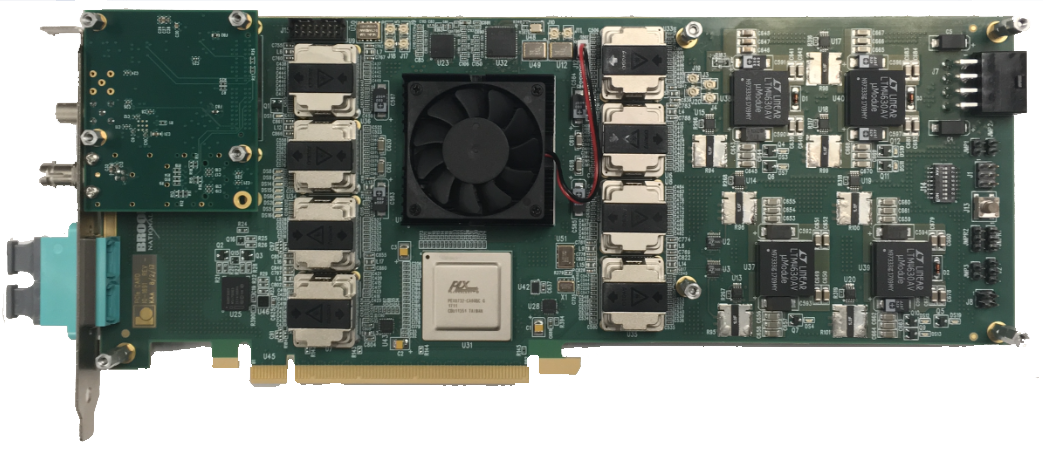
\includegraphics[width=1.5cm]{figs/felix.png}};
	\draw [thick,rounded corners=2pt] (-0.9,0.9)  rectangle (0.9,-0.1);
	\draw (-0.1,0.2) node {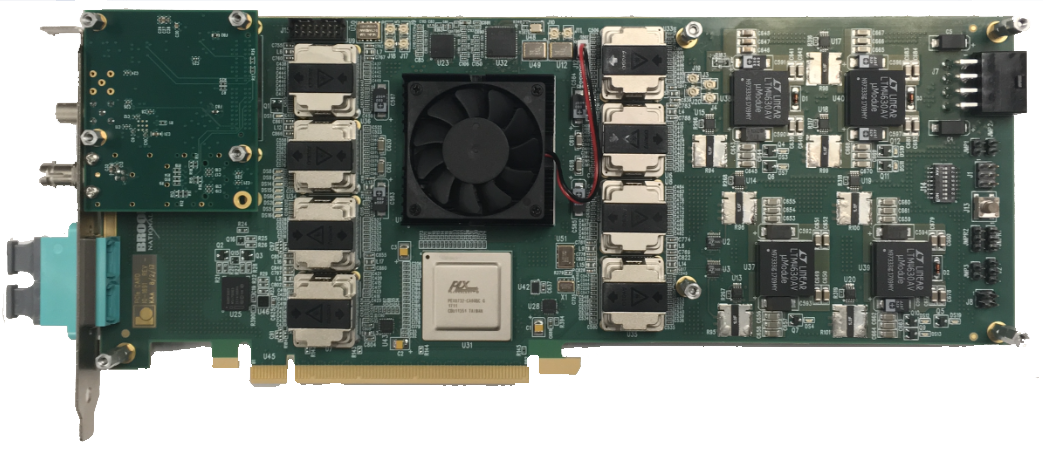
\includegraphics[width=1.5cm]{figs/felix.png}};
	\draw [thick,rounded corners=2pt] (-0.9,-.2)  rectangle (0.9,-1.2);
	\draw (-0.1,-0.9) node {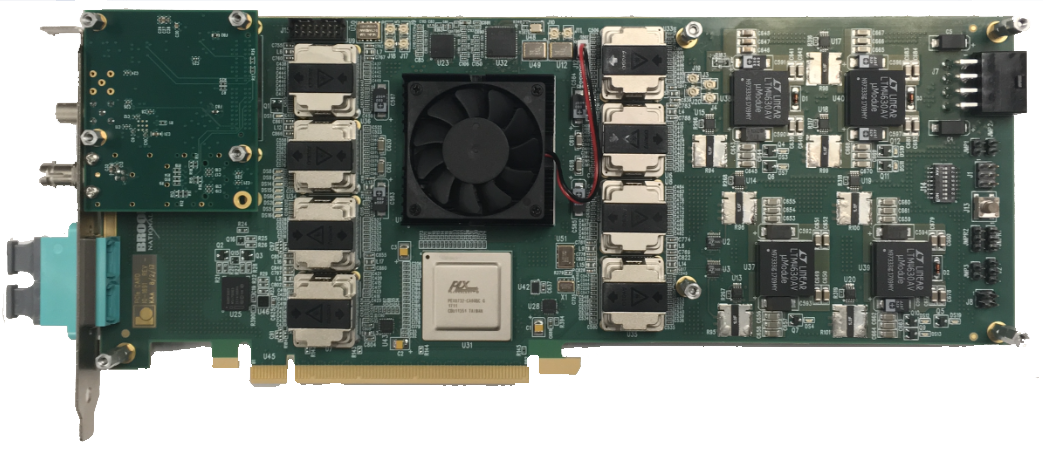
\includegraphics[width=1.5cm]{figs/felix.png}};
	\fill (-0.3,-1.6) circle(0.075);
	\fill (0,-1.6) circle(0.075);
	\fill (0.3,-1.6) circle(0.075);
}
}

{\sffamily
\begin{tikzpicture}     
  \draw (-3,0) node[]{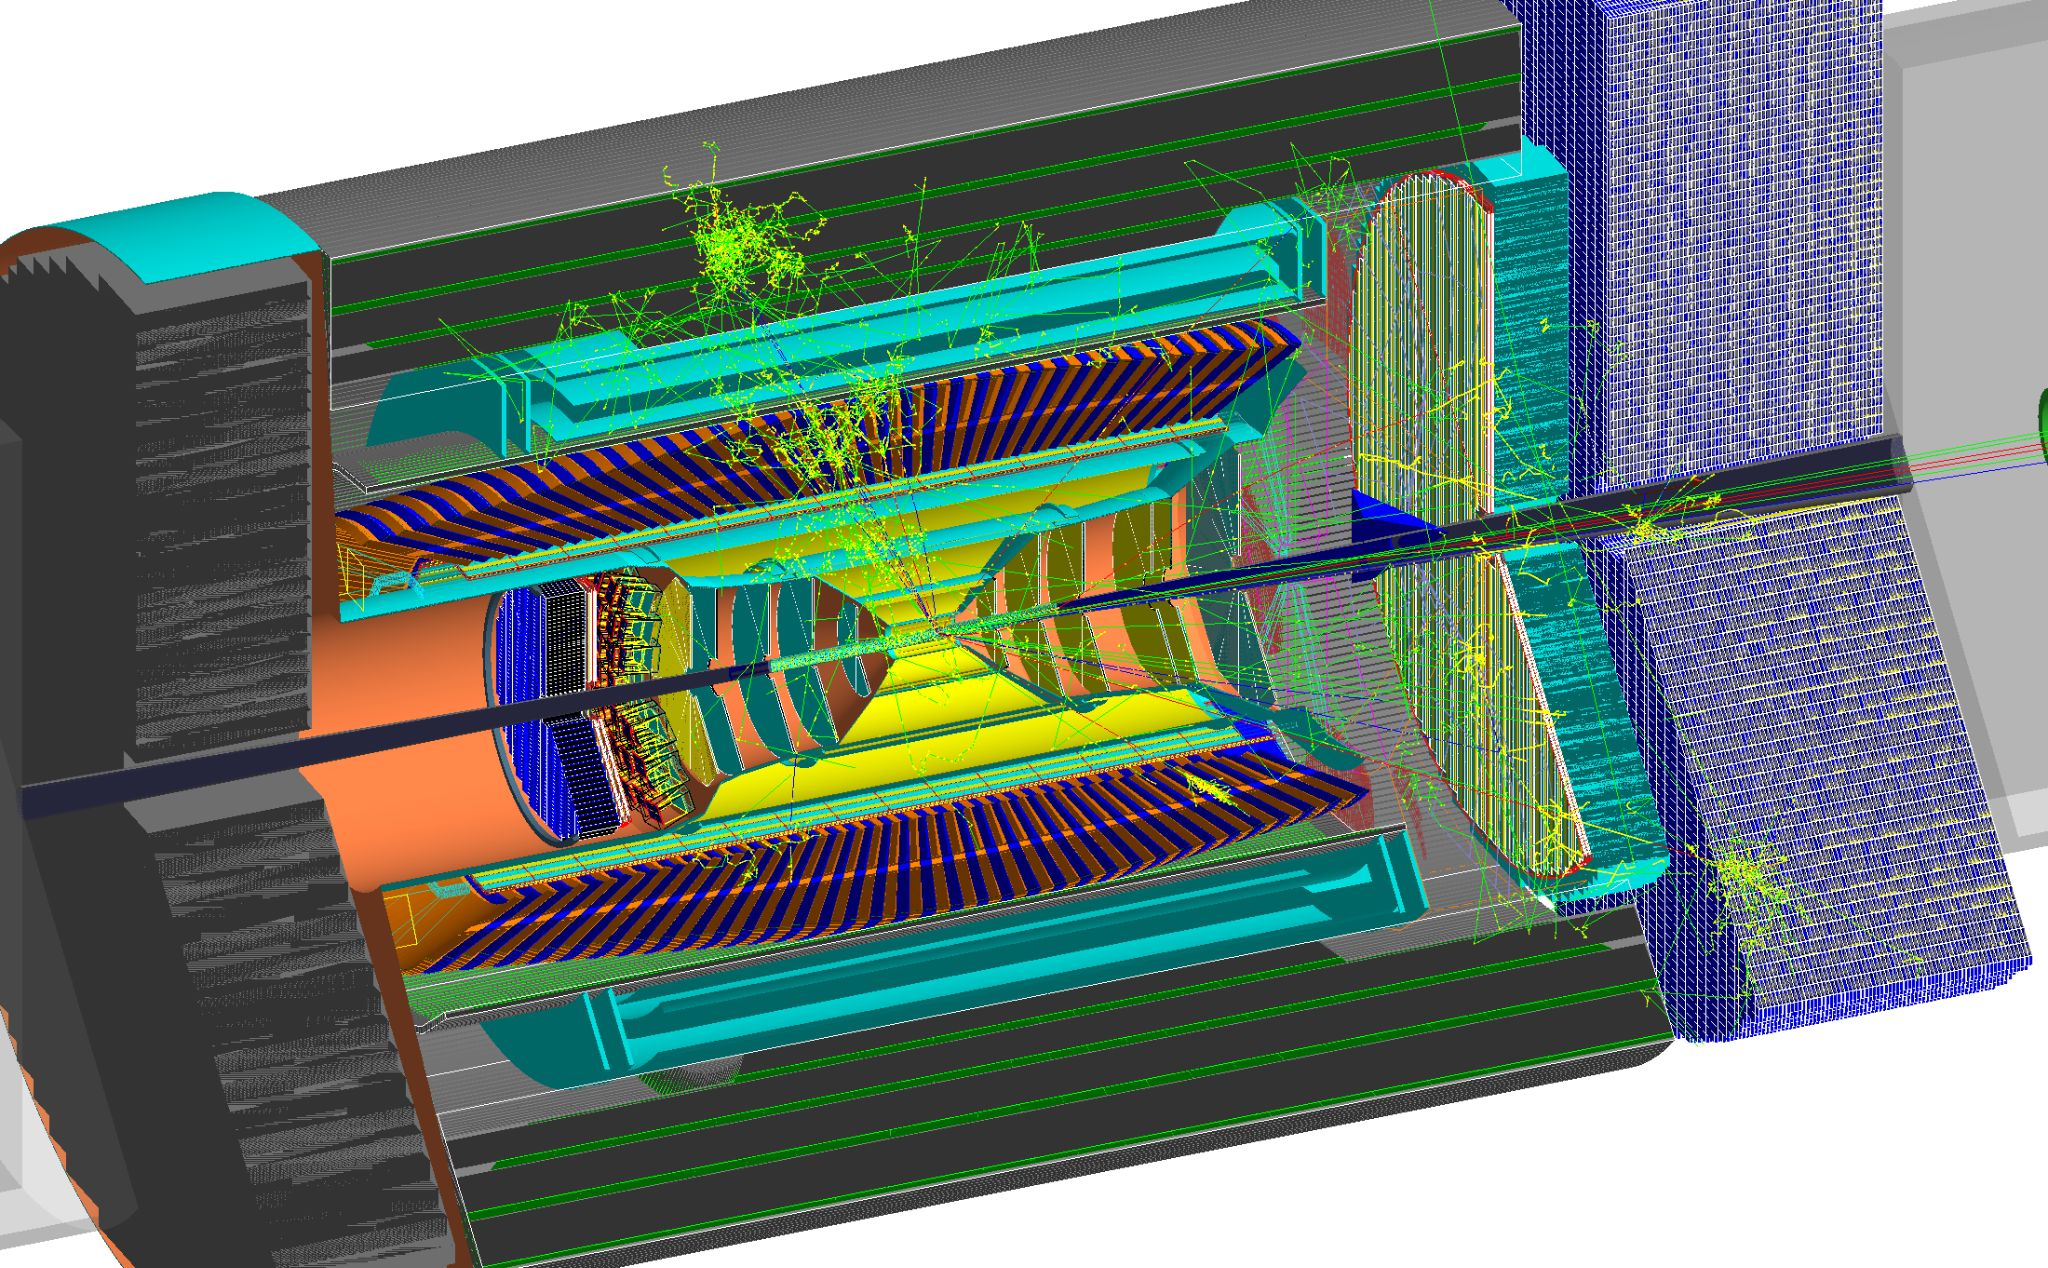
\includegraphics[width=3cm]{figs/detector.jpg}};   

\draw[locality] (-3,3) node {\large Detector};
\draw[locality] (1.5,3) node {\large Exp.~hall};
\draw[locality] (5.9,3) node {\large Counting room};
\draw[locality] (10.2,3) node {\large on-site/off-site};

\draw[locality,dashed,very thick] (-0.3,2.5) -- (-0.3,-5);
\draw[locality,dashed,very thick] (3.3,2.5) -- (3.3,-5);
\draw[locality,dashed,very thick] (8.3,2.5) -- (8.3,-5);



\draw[fiber] (-1.3,1.9) -- (4,1.9);
\draw[fiber] (-1.3,1.7) -- (4,1.7);
\draw[fiber] (-1.3,1.5) -- (4,1.5);
\draw[fiber] (-1.3,1.3) -- (4,1.3);

 \pic at ( -1.6 , 2.0) {fee};
 \pic at ( -1.4 , 1.8) {fee};
 \pic at ( -1.2, 1.6) {fee};
 \pic at ( -1 , 1.4) {fee};


\draw[fiber] (-1.3,0.2) -- (2.3,0.2);
\draw[fiber] (-1.3,0.) -- (2.3,0);
\draw[fiber] (-1.3,-.2) -- (2.3,-0.2);
\draw[fiber] (-1.3,-.4) -- (2.3,-.4);
\draw[fiber] (2.5,-0.1) -- (4,-0.1);
 \pic at ( -1.6 , 0.3) {fee};
 \pic at ( -1.4 , 0.1) {fee};
 \pic at ( -1.2, -0.1) {fee};
 \pic at ( -1 , -0.3) {fee};
  


\draw(-1.3,-1.5) -- (0.3,-1.5);
\draw(-1.3,-1.7) -- (0.3,-1.7);
\draw (-1.3,-1.9) -- (0.3,-1.9);
\draw(-1.3,-2.1) -- (0.3,-2.1);
  
\draw[fiber] (0.7,-1.6) -- (4,-1.6);
 \pic at ( -1.6 , -1.4) {fee};
 \pic at ( -1.4 , -1.6) {fee};
 \pic at ( -1.2,-1.8) {fee};
 \pic at ( -1 , -2) {fee};

\pic at (0.5,-1.75) {fep};

\pic at (2.5,-0.075) {sag};

\pic at (5,0) {rackwfelix};
\pic at (7.1,0) {rack};
\pic[scale=0.5] at (6.75,-3.05) {disc};
\draw  (6.75,-3.4) node[anchor=north]{\small Local buffer};
\draw[thick, rounded corners=3pt,fill=monitoring] (4,-4.6) rectangle (7.75,-5.4);
\draw (5.875,-5.) node {\small Monitoring};


\pic[scale=0.5] at (9.5,-0.6) {disc};
\pic[scale=0.5] at (9.5,-0.3) {disc};
\pic[scale=0.5] at (9.5,0.) {disc};
\pic[scale=0.5] at (9.5,0.3) {disc};
\pic[scale=0.5] at (9.5,0.6) {disc};

\pic[scale=0.5] at (10.75,-0.6) {disc};
\pic[scale=0.5] at (10.75,-0.3) {disc};
\pic[scale=0.5] at (10.75,0.) {disc};
\pic[scale=0.5] at (10.75,0.3) {disc};
\pic[scale=0.5] at (10.75,0.6) {disc};



\draw[implies-implies,double distance=0.15cm] (7.7,-0.1) -- (8.9,-0.1);

\draw[implies-implies,double distance=0.15cm] (6.75,-2) -- (6.75,-2.85);

\draw[-implies,double distance=0.15cm] (6.75,-3.9) -- (6.75,-4.6);
\draw[-implies,double distance=0.15cm] (5.0,-2.1) -- (5.0,-4.6);


\draw (1,2.1) node {\small Fiber};
\draw(-0.5,-2.7) node {\small LVDS $\mathcal{O}$(5)m};
\draw(-0.5,-3.1 ) node {\small analog $\mathcal{O}$(20)m};

\pic[scale=0.5] at (9.5,-3.5) {smallrack};
\pic[scale=0.5] at (10.5,-3.5) {smallrack};
\pic[scale=0.5] at (11.5,-3.5) {smallrack};

\draw[implies-implies,double distance=0.15cm] (9.5,-1.1) --(9.5,-2.4);
\draw[implies-implies,double distance=0.15cm] (10.75,-1.1) --(10.75,-2.4);
\draw (10.5,-5) node{\small  JLAB,SDCC, OSG, ...};

\end{tikzpicture}
}
  
  \caption[Data Acquisition Diagram]{\label{fig:data_acquisition_diagram} The DAQ electronics deployment can be roughly divided by their location, with Front End Electronics (FEE) modules on/near the detector; Front End Processor boards (FEP) which digitize or reformat detector information and Stream Aggregator Boards (SAB), which bundle streams, in the hall; and online filtering and monitoring in the counting room. Long term storage and analysis processing is performed in a federated model on multiple sites. }
  %\caption[Data Acquisition Diagram]{\label{fig:data_acquisition_diagram} Diagram of a Data Acquisition system. This is reproduced from slides shown at AI4EIC 2021\cite{EIC_readout_overview_AI4EIC_2021}. }
 \end{center}
\end{figure}


\subsection{DAQ components}
 Front-end electronics (FEE) modules sit inside or on the detector. In most cases, detector-specifc ASICs provide the data conversion from the analog to digital domain, do zero-suppression and provide an interface to fiber transceivers for data transport to the counting room.  There, we envision FELIX-type PCIe-based receiver cards\footnote{In the following, we will use "FELIX card" as a stand-in for a successor board of similar architecture.} which support a large number of high speed fiber links per card.  

Since some FEE may not utilize the full bandwidth of a fiber link, cost-effective stream aggregator boards (SABs), based either on small FPGAs or COTS multiplexer ICs, can bundle multiple fiber links coming from FEE to a single fiber to the FELIX cards. 

Because of space and services constraints, or because no suitable ASIC is available, some FEEs will connect to Front end processor (FEP) modules via digital (LVDS) or analog links. The FPGA and possibly analog to digital converter logic on the FEP will then generate a data stream suitable for fiber transport to the FELIX cards.

In the counting room, we expect a number of special servers which house the FELIX cards. Each FELIX/CPU combination sees data from a certain subset of detector channels and can do additional data reduction before sending out the data to the counting room CPU farm. This CPU farm (with possibly GPU accelerators) will do further data reduction, for example via high level data selection algorithms.

The data streams are buffered on local hard disks, with enough capacity to store the data for several days. This local buffer has multiple functions: 
\begin{itemize}
    \item It averages out the changes in data rate from luminosity changes so that the upstream link only need to provide average, not peak, bandwidth.
    \item It allows stand-alone operation for a limited time when the data transport out of the counting house is not available or runs at reduced capacity.
    \item It allows for near-online monitoring and replay of recent data for quality control, especially for those quantities which depend on on-going calibrations.        
\end{itemize}

The data are then pushed upstream to on-site or federated storage as part of the overall EIC project.

\subsection{Online monitoring}\label{subsec:online_mon}
Online monitoring is divided into a fast path with bound latency and a slow path. The fast path provides low-latency feedback for accelerator steering and equipment protection. The data for this path are generated early in the DAQ chain, either on the FELIX host CPUs or on the FELIX card themselves. Necessarily, they are limited in scope to counting, summing or similar type of information. The slow path provides higher-level information for quality control. Here, it's possible to reconstruct and analyse full events on-the-fly, by copying pre-selected time segments from the data stream to the analysis sub-cluster. Note here that such a monitoring system does not require the guaranteed reconstruction of all data, just of a suitable subset. That subset can either be selected unbiased by selecting periodic time segments, or biased by selecting time-segments tagged by data filters in the main data stream.  Similar monitoring can be performed on data on the local buffer for those quantities which require calibration data or two-pass analysis.

% DL
For both types of data a system will be needed to evaluate the monitoring data and inform the experiment operators of potential issues. This will largely include the creation of histograms which may be monitored either graphically or by some automated means. The prevalence of AI will certainly play a large role in that it will be able to evaluate a wider variation of monitoring data and at a much higher rate than could be expected of humans. Such systems are already deployed and under development~\cite{Hydra2021}. 

\subsection{Risk mitigation}
We expect that during initial commissioning noise rates will be significantly higher than during established operation, as accelerator and detector parameters will not yet be tuned optimally. Such high noise rates might overwhelm processing and upstream write capability. To allow progress in this initial phase, the DAQ system will allow to input a bounded-latency signal on the FELIX card or host CPU level to suppress uninteresting time segments.

Such a system also allows us to simply incorporate a dedicated collision detector for rate reduction: only time segments which are flagged to have a collision are kept, others are dropped early in the processing chain. 

This bounded-latency system could either be realized as a classic hardware filtering signal, or via software messages sent to the FELIX hosts with a clear advantage with regard to flexibility and ease of implementation, but with possibly a larger latency. The optimal implementation depends on the capabilities of the future FELIX successor and bandwidth availability on the FELIX host servers.

\subsection{AI-based data selection}

Traditionally, online data selection is performed using fixed topological cuts such as an energy deposit threshold in a calorimeter or the minimum transverse momentum of a track. Online data selection can benefit from the introduction of ML techniques typically used in offline data selection. It is advantageous to introduce these techniques at this stage to keep events that would be rejected by conventional methods and thereby increasing the overall physics output of a detector. This approach can also simultaneously reject events that have a level of noise that would render a physics analysis of this event impractical.

The consortium is constructing a system where these selection techniques can be realised directly in hardware and will initially be deployed at sPHENIX which will double as a test system for an EIC detector. This project involves two symbiotic AI systems; one to identify collisions containing heavy flavor decays through their unique topology and another to determine the beamspot for the detector during operation. The latter system then feeds back to the data selection system to improve the physics efficiency.


%There are several features of these decays which separate them from background such as tracks which do not point to the collision vertex, tracks which meet at a point away from the collision vertex (characteristic of the secondary vertex) and an overall increase in the number of tracks. It is possible that not all signatures of these decays are present in each signal candidate and so conventional selections tend to have a large number of background candidates by having sufficiently loose selections to overcome this. This situation is also worsened by the relatively small cross-sections for heavy flavor production compared to minimum bias collisions, there are approximately 50 background candidate for each $c\bar{c}$ pair produced~\cite{jackson2016measurement, aaij2013prompt}. Using AI to select these decays over conventional methods has the ability to drastically improve the signal-to-background ratio for several physics channels and, in a test case using simulated $D^0\rightarrow K^-\pi^+$ decays\footnote{charge-conjugation is implied} and background collisions, it was found that an untuned machine learning algorithm was able to increase the background rejection from 57.4$\,\pm\,$4.2$\%$ to 73.3$\,\pm\,$3.7$\%$ for comparable signal efficiencies (81.2$\,\pm\,$3.5$\%$ for the conventional method and 79.3$\,\pm\,$3.6$\%$ for the AI-based data selection). This test example was simulated using the sPHENIX detector which shares many similarities with the ECCE detector and it is expected that the background rejection can be improved with careful tuning of algorithms.

In the system, the accept decisions would be handled by a separate FELIX system which aggregates information from several subdetectors but it should be noted that the choice of technology could evolve along with general hardware developments in the next decade. The FELIX has 48 bi-directional links allowing for data from multiple systems to be passed to a single FELIX board. The machine learning algorithm will then be loaded onto the FPGA which will be capable of basic tracking (using tracklets from the vertex, sagitta and FST detectors) to make decisions that can be fed back to the initial DAQ or global data selection system to signal processing should continue. This should be achieved within 6$\,\mu$s\footnote{This requirement is determined by the shaping time of sPHENIX's vertex detector and could differ for ECCE}. The sPHENIX-based system will be restricted to using information from the trackers. Heavy flavor decays can also leave significant deposits in the calorimetry system but this is limited to 15\,kHz at sPHENIX. If this bottleneck can be remedied for ECCE, the selection system can be improved further. %Block diagrams of the FELIX board when used as a data selection system with the relevant data paths are given in Figure~\ref{fig:felix-ai}.

%\begin{figure}[hbt!]
%	\begin{center}
%		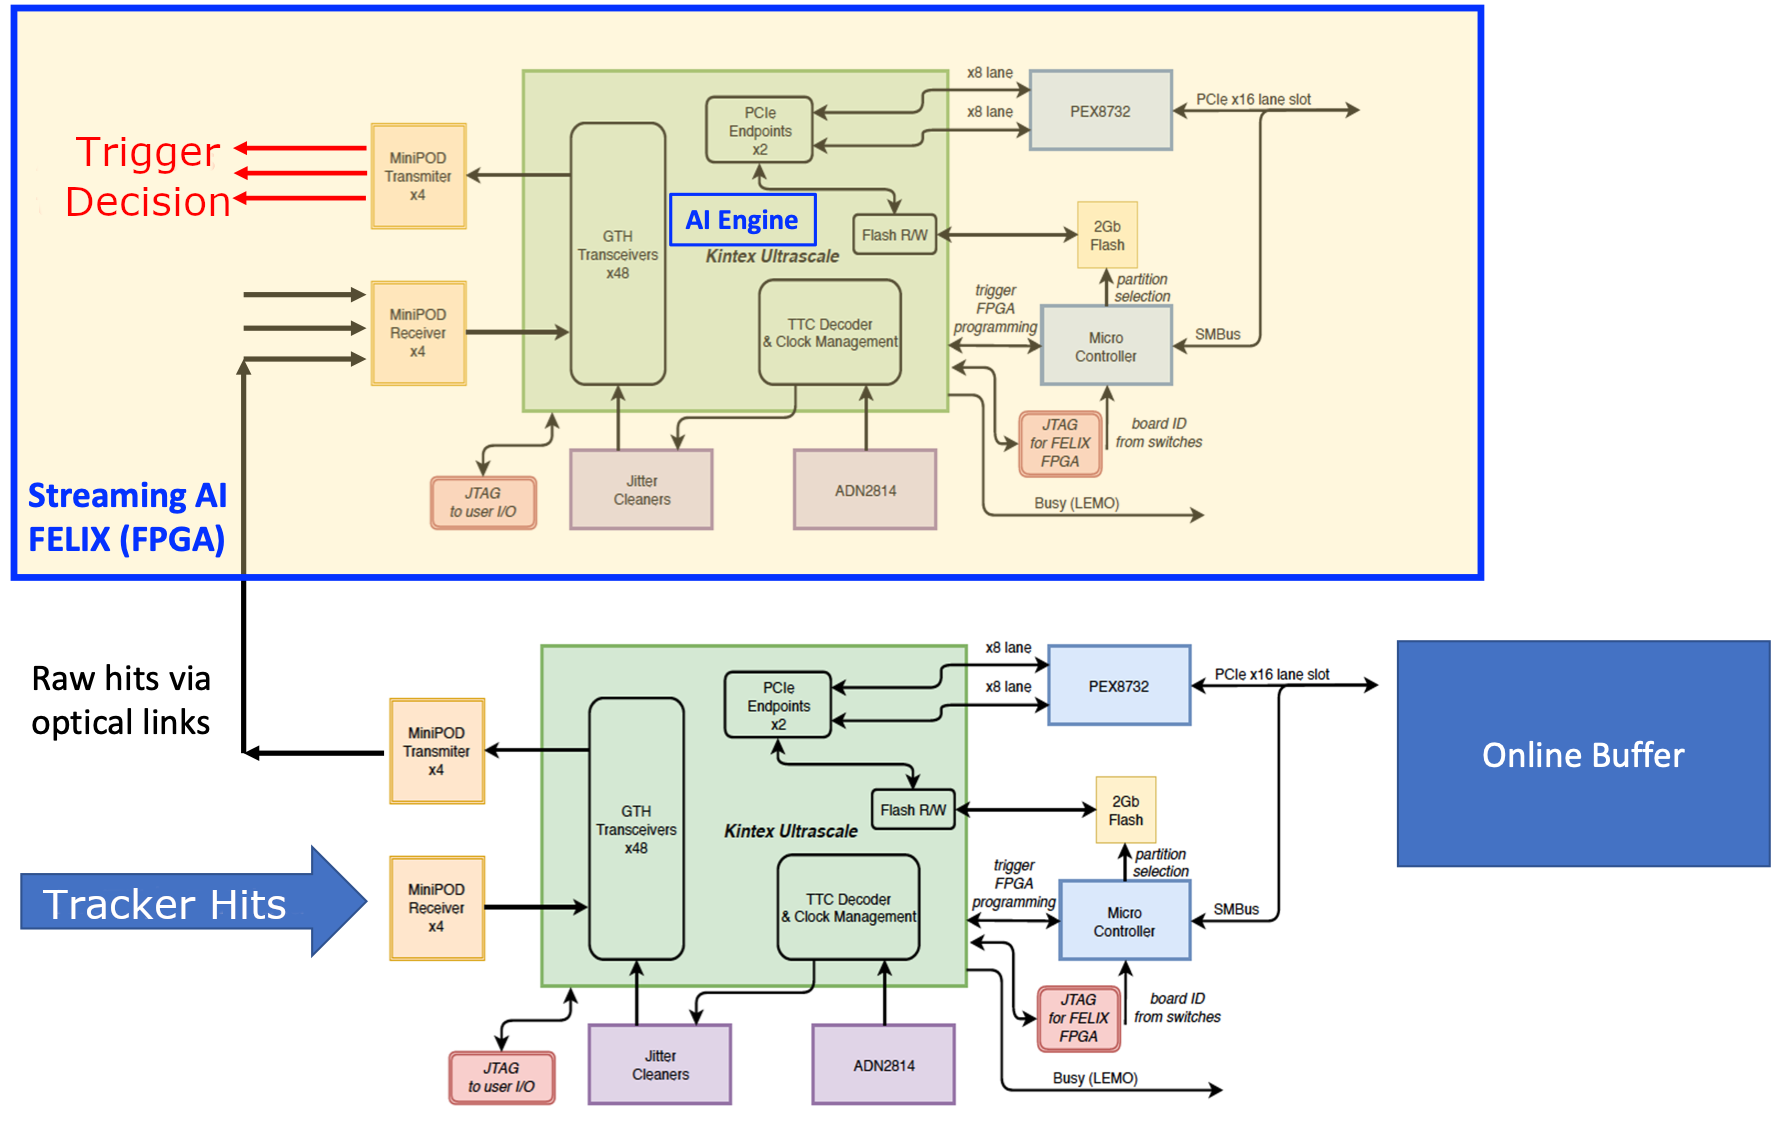
\includegraphics[width=0.8\textwidth]{figs/FELIX-AI}
%		
%		\caption[FELIX data selection System]{Block diagram of two FELIX boards when used as in the proposed smart data selection system. The FELIX on the bottom represents the conventional DAQ system that aggregates from subsections of the tracking system. There can be many of these systems. The top FELIX acts as the selection system, taking data from multiple systems and gives a single decision for each collision passed to it. The system combines the data and the Kintex Ultrascale contains GNNs capable of fast tracking and data selection.}\label{fig:felix-ai}
%	\end{center}
%\end{figure}

Studies are ongoing, comparing the outputs of algorithms trained using Convolution Neural Networks (CNNs) and Graph Neural Networks (GNN). For many applications, GNNs often represent a more robust ML algorithm than CNN due to using additional information from the edges of the graph as well as the node information used by a traditional CNN. This makes them more applicable to sparse data such as tracking and data selection where the overall occupancy of the detector system is low.

It is important to note that the beam conditions can change with time, this can be both during a run and on a longer scale. Thus it is imperative that, as well as developing a selection algorithm, we develop a feedback system that is capable of monitoring the beam conditions in real time and adapting the input parameters to this. For example, the position of the collision point directly impacts the measurement of the track displacement. If this moves, it will alter the signal and background efficiencies in opposite directions. This monitoring will be achieved using GPUs which will feedback to the selection system. GPUs typically perform well using CNNs which motivates the study of various machine learning methods to find the optimal set of algorithms to use for each stage of the selection and monitoring. Other important features that can appear in a detector, impacting this system and hence must be monitored are the appearance of noisy channels (or pixels) and displacement of parts of the detector, such as through thermal expansion or vibrations. It has been demonstrated that algorithms can run fast enough on GPUs to achieve this form of monitoring~\cite{gpu2021}.


%The project was approved in August 2021 and development of the algorithm is underway using simulated signal and background collisions. The algorithm will be translated for loading onto the FPGA using hls4ml~\cite{fahim2021hls4ml} and testbenches have been set up using 2 Xilinx development boards; a KC705 and VC709, the latter of which shares the same FPGA as the FELIX board. The KC705 will read simulated hits, in the same data format as the real detector, and send it to the VC709 via optical links and thus the KC705 emulates the DAQ and the VC709 emulates the selection system. The hls4ml package has already demonstrated the ability to translate ML algorithms to high level synthesis language which can be transferred to an FPGA as a bitstream and the stages required are shown in Figure~\ref{fig:hls4ml}. It has also been shown that the KC705 can receive data from host-to-client using Direct Memory Access (DMA). This project has been funded for two fiscal years and will use sPHENIX as a proof-of-principle. sPHENIX will cease operations before ECCE data taking and thus a smart data selection system is a realistic prospect for ECCE.


%\begin{figure}[hbt!]
%   \begin{center}
 %       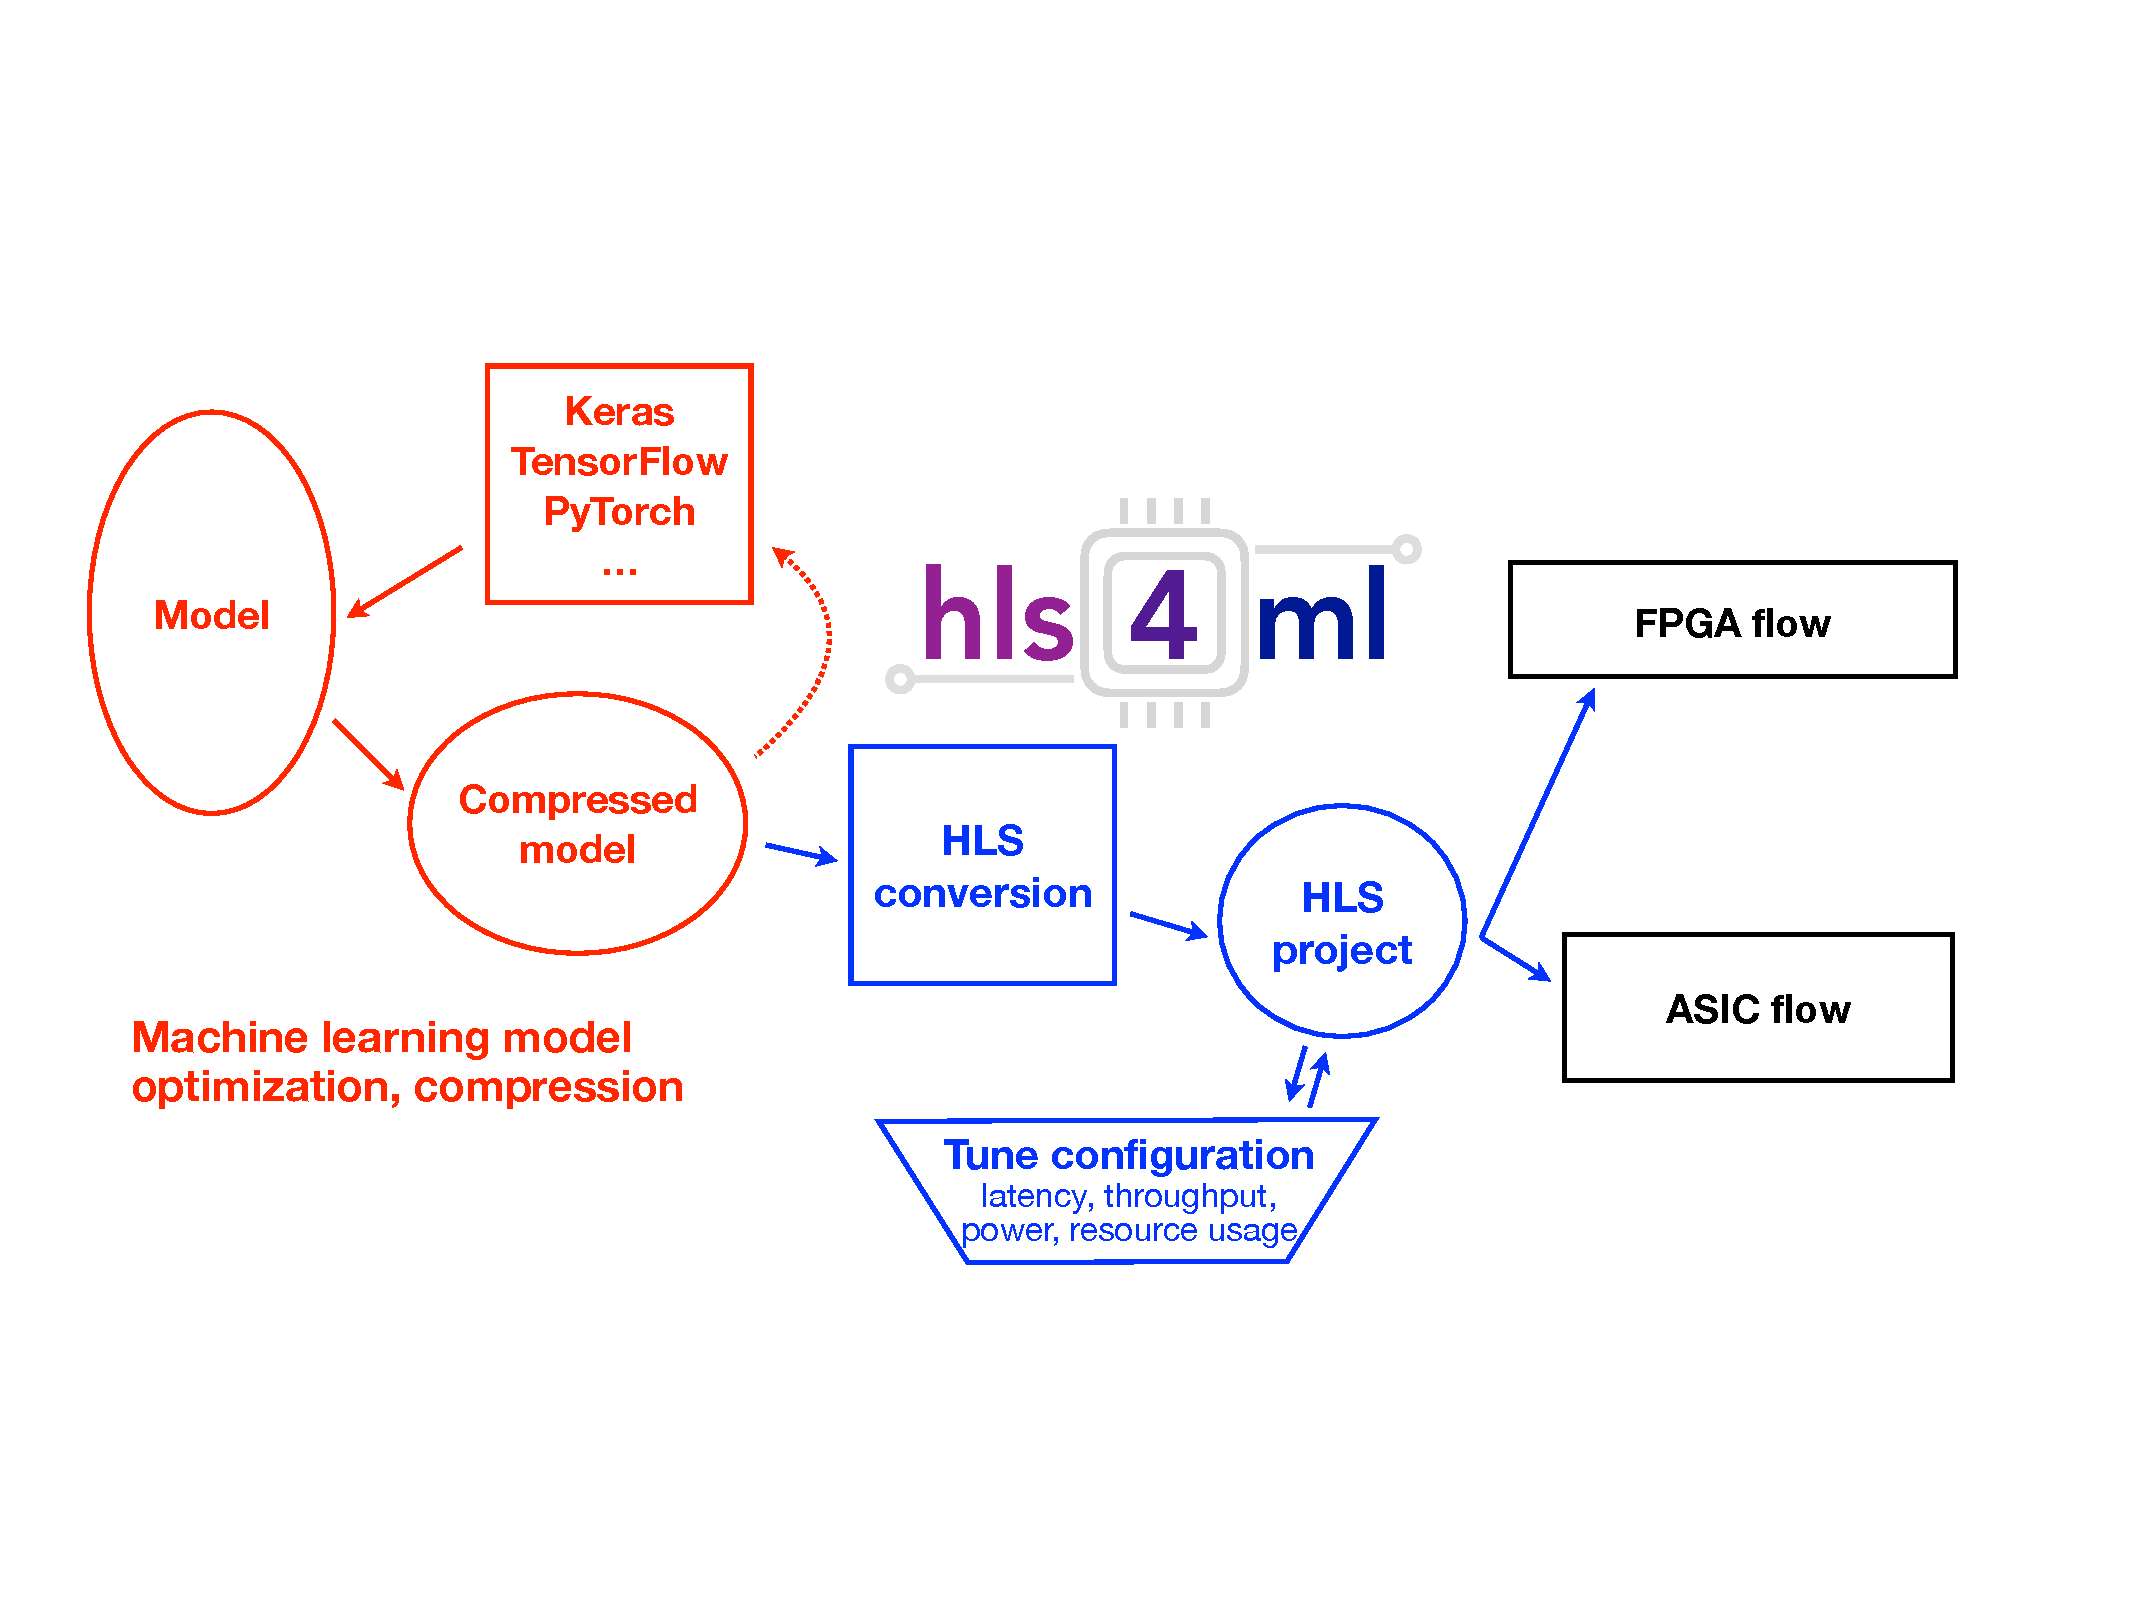
\includegraphics[width=0.8\textwidth]{figs/hls4ml-flow-4}
%        
 %       \caption[hls4ml workflow]{The workflow for converting a ML algorithm to a firmware block. The red sections represent the conventional AI development stages, the blue sections represent the conversion to HLS language and the black sections represent the output options.}\label{fig:hls4ml}
 %   \end{center}
%\end{figure}



\subsection{Expected data rates and reduction steps}

%\emph{JCB: I'm not sure how valid these numbers are.}

Since connections between detector and FEPs might not be zero-suppressed digital or even analog data, it makes no sense to specify a data rate at the detector-to-hall border. Instead, the following section describes the expected data rate on the Fiber/FELIX level and downstream from there.

At nominal luminosity, we expect that true signals and beam-gas interactions produce a total rate of $\mathcal{O}$(100 Gbps) of zero-suppressed data at the FELIX card level. However, detector noise and additional backgrounds, especially during early operation, can completely dominate this rate. We assume therefore a total rate of $\mathcal{O}$(10 Tbps) bandwidth on the fiber level. Next-gen FELIX cards will have 25 Gbps receivers; for headroom for burst rates, non-ideal allocation of detector channels to fibers \emph{etc.}, we assume 12.5 Gbps as the average rate per fiber, and as a consequence, about 800 fibers.

A current-generation FELIX card has 48 fiber ports, leading to $\mathcal{O}$(20) FELIX cards. Each card would then receive 600 Gbps. We assume that at the time of procurement for EIC, cards based on at least PCIe Gen5 are available, providing 500 Gbps to the host server, requiring a modest reduction of the data rate in FELIX card itself, for example via cross-channel noise reduction. In combination with the host CPU, we expect a total reduction by a factor of 5 to $\mathcal{O}$(2) Tbps total, 100 Gbps per server. We note that a typical server with 128GB of memory can buffer the full stream for about 2 seconds, ample time for region-of-interest/time-slice-of-interest communication between the FELIX hosts, making higher reduction factors comparatively easy to achieve. The data can then be streamed out via a dual 100 Gbps link to the second layer in the compute farm.

In the compute farm, the data is further analyzed and filtered. We expect that with inter-detector noise suppression and high-level data selection the required effective bandwidth to long-term storage can be reduced to $\mathcal{O}$(100) Gbps.  



%--------------------------------------------------------------------



